\subsubsection{\Suspension}\label{ssec:designdims:suspension}

\begin{figure}[t]
  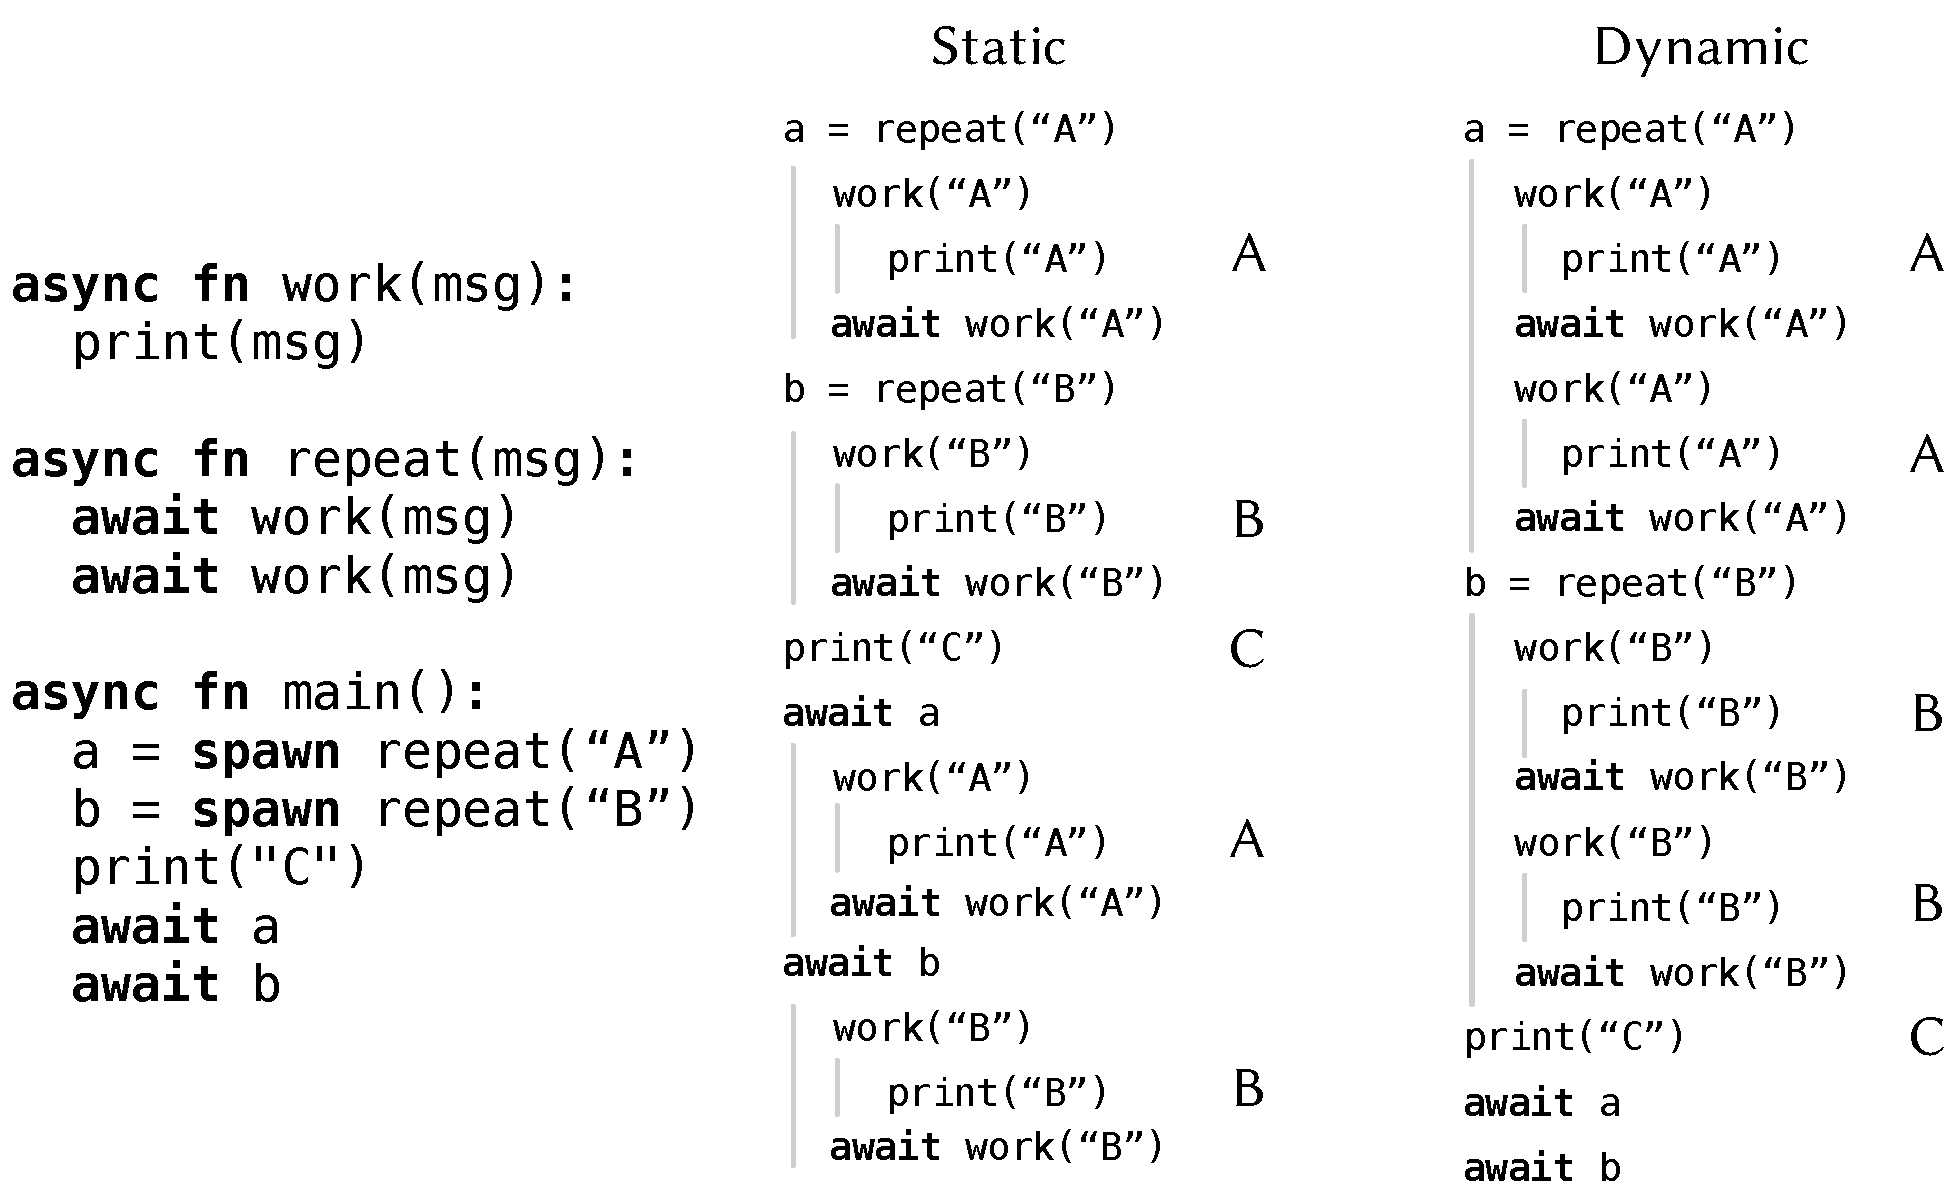
\includegraphics[width=0.7\linewidth]{f/suspension.pdf}
  \caption{An example program demonstrating the \Suspension dimension, executed with \Js (\static) and \CSharp (\dynamic). Each column shows an execution trace of the program under an eager semantics with each kind of \suspension. The execution traces are nested according to their level in the call stack, and the order of prints to stdout is emphasized in the right part of each column.}
  \label{fig:suspension}
\end{figure}

Once asynchronous work has started, the next design divergence occurs at await points. The \Suspension dimension defines the guarantees a language makes about whether an await point is guaranteed to yield control. For example, consider the program in \Cref{fig:suspension} executing under an \eager semantics. The line \code|a = repeat("A")| will call into \code|work("A")| which will call \code|print("A")| and return to \lstinline[language=Pseudo]|await work("A")|. The task for \code|work("A")| has been completed, so a language has two choices: either yield control to the caller, or continue evaluation past the \lstinline[language=Pseudo]|await|. We call the former strategy \emph{\static} suspension because an await point is statically guaranteed to always yield. We call the latter strategy \emph{\dynamic} suspension because whether an await point yields depends on the awaited task.

In only one language surveyed, \Js, an await point is guaranteed to yield according to the ECMAScript specification \cite[\textsection 27.7.5.3, step 3.b]{ecma_ecmascript_nodate}. Therefore in \Cref{fig:suspension}, running under \Js semantics, the program outputs ``ABCAB'' because \lstinline[language=Pseudo]|await work("A")| yields back to \code|main|. In all other languages, no such guarantee exists. For the example program operating under an eager semantics such as in \CSharp, the program would output ``AABBC'' because \lstinline[language=Pseudo]|await work("A")| observes that \code|work("A")| is complete and therefore the await expression can continue evaluation.

\paragraph{Design rationale.}

The principal reason to adopt \static suspension is to prevent starvation. Under an eager approach with \dynamic suspension, if a compute-bound task is called before calling \abbr{i/o}-bound tasks, the first task can starve the remaining tasks of CPU time. A \static suspension policy reduces the likelihood of that compute-bound task never yielding control back to the executor.

\Static suspension comes at a performance cost. In the case of awaiting a completed task, \static suspension requires a round-trip to the runtime and back to continue past the await. Languages with \dynamic suspension can mitigate the starvation issue by providing a \code|yield_now| primitive which has no effect but to yield control to the runtime.

